\documentclass[11pt,a4paper]{article}
\usepackage[T1]{fontenc}
\usepackage[utf8]{inputenc}
\usepackage{lmodern}
\usepackage[margin=2cm]{geometry}
\usepackage{xcolor}
\usepackage{listings}
\usepackage{booktabs}
\usepackage{tabularx}
\usepackage{array}
\usepackage{enumitem}
\usepackage{tikz}
\usepackage{amsmath,amssymb}
\usepackage{fancyhdr}
\usepackage{titlesec}
\usepackage[hidelinks]{hyperref}

\definecolor{ok}{RGB}{30,130,60}
\definecolor{bad}{RGB}{190,40,40}
\definecolor{part}{RGB}{200,120,0}
\definecolor{none}{RGB}{120,120,120}
\definecolor{codebg}{RGB}{246,246,246}
\definecolor{accent}{RGB}{30,70,140}

\lstset{language=Python, basicstyle=\ttfamily\small, backgroundcolor=\color{codebg},
  keywordstyle=\color{accent}\bfseries, commentstyle=\color{none}\itshape,
  stringstyle=\color{ok}, showstringspaces=false, frame=single, rulecolor=\color{codebg},
  columns=fullflexible, keepspaces=true, breaklines=true, numbers=left, numberstyle=\tiny\color{none},
  xleftmargin=1.5em, framexleftmargin=1.5em}

\newcommand{\sq}{\textquotesingle}
\newcommand{\pts}[3]{\fcolorbox{#3}{white}{\color{#3}\textbf{#1\,/\,#2}}}
\newcommand{\OK}{\textcolor{ok}{\textbf{correct}}}
\newcommand{\PART}{\textcolor{part}{\textbf{partially correct}}}
\newcommand{\NONE}{\textcolor{none}{\textbf{not attempted}}}
\newcommand{\boxnote}[2]{\par\smallskip\noindent\fcolorbox{#1}{white}{\parbox{\dimexpr\linewidth-2\fboxsep-2\fboxrule}{#2}}\par\smallskip}

\titleformat{\section}{\Large\bfseries\color{accent}}{\thesection}{0.6em}{}
\titleformat{\subsection}{\large\bfseries}{\thesubsection}{0.6em}{}
\pagestyle{fancy}\fancyhf{}
\lhead{\small CSC\_2F002\_EP --- Mock midterm (sorting networks \& game trees) --- correction}
\rhead{\small \thepage}
\setlength{\headheight}{14pt}
\setlength{\parindent}{0pt}
\setlength{\parskip}{0.45em}
\sloppy

\begin{document}

%======================================================================== FRONT PAGE
\begin{center}
{\LARGE\bfseries Mock midterm --- Correction report}\\[0.3em]
{\large Sorting networks (divide and conquer) \& evaluating game trees (randomisation)}\\[0.2em]
{\small Graded on the correctness of the algorithms (not on test results), partial credit allowed,
point values of the statement (20 in total). Version graded: \texttt{networks.py} of 25 Nov., 12:28;
\texttt{gametree.py} unchanged since the download.}
\end{center}

\vspace{0.3em}
\begin{center}
\fcolorbox{accent}{white}{\parbox{0.5\linewidth}{\centering
{\large Final grade}\\[0.2em]
{\fontsize{34}{38}\selectfont\bfseries\color{accent} 3.25 / 20}\\[0.2em]
{\small 16.25\,\%}\\[0.1em]{\small Problem 1: 3.25\,/\,10 \qquad Problem 2: 0\,/\,10}}}
\end{center}

\vspace{0.2em}
\begin{minipage}[t]{0.47\linewidth}
\textbf{Points per question}\\[0.3em]
\small
\begin{tabular}{@{}llrr@{}}
\toprule
Q & Function / answer & Pts & Max\\
\midrule
1 & \texttt{apply\_network} & \textcolor{ok}{1} & 1\\
2 & bitonic test, 0-1 principle & \textcolor{part}{1.25} & 2\\
3 & bubble network + count & \textcolor{ok}{1} & 1\\
4 & half-cleaner, merger, $M(n)$ & \textcolor{none}{0} & 4\\
5 & bitonic sorter, $S(n)$, $D(n)$ & \textcolor{none}{0} & 2\\
\midrule
6 & \texttt{eval\_full} + complexity & \textcolor{none}{0} & 1\\
7 & left first, \texttt{worst\_case} & \textcolor{none}{0} & 2\\
8 & \texttt{eval\_random} & \textcolor{none}{0} & 2\\
9 & bounds $a_k, b_k$, $O(n^c)$ & \textcolor{none}{0} & 3\\
10 & budget, Monte Carlo & \textcolor{none}{0} & 2\\
\midrule
 & \textbf{Total} & \textbf{3.25} & \textbf{20}\\
\bottomrule
\end{tabular}
\end{minipage}\hfill
\begin{minipage}[t]{0.5\linewidth}
\textbf{Earned (filled) vs available (outline)}\\[0.3em]
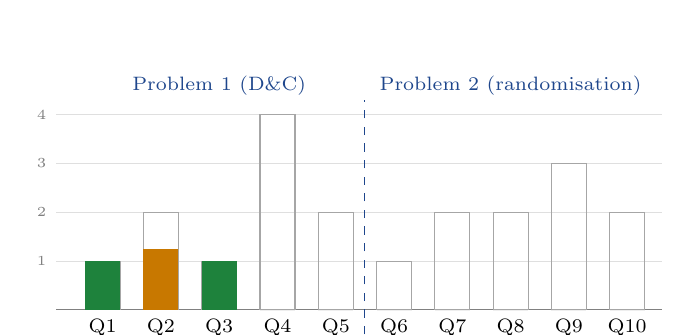
\begin{tikzpicture}[x=0.74cm,y=0.62cm]
  \foreach \y in {1,2,3,4} {\draw[gray!25] (0.2,\y) -- (10.6,\y); \node[left,font=\tiny,gray] at (0.2,\y) {\y};}
  \draw[gray] (0.2,0) -- (10.6,0);
  \foreach \q/\m/\e/\c in {1/1/1/ok, 2/2/1.25/part, 3/1/1/ok, 4/4/0/none, 5/2/0/none,
                           6/1/0/none, 7/2/0/none, 8/2/0/none, 9/3/0/none, 10/2/0/none} {
    \draw[gray!70] (\q-0.3,0) rectangle (\q+0.3,\m);
    \fill[\c] (\q-0.3,0) rectangle (\q+0.3,\e);
    \node[below,font=\scriptsize] at (\q,0) {Q\q};
  }
  \draw[dashed,accent] (5.5,-0.5) -- (5.5,4.3);
  \node[font=\scriptsize,accent] at (3,4.6) {Problem 1 (D\&C)};
  \node[font=\scriptsize,accent] at (8,4.6) {Problem 2 (randomisation)};
\end{tikzpicture}
\end{minipage}

\vspace{0.6em}
\textbf{Metrics}\\[0.2em]
\small
\begin{tabularx}{\linewidth}{@{}Xr@{\qquad}Xr@{}}
\toprule
Functions written (of 14 asked) & 4 / 14 & Fully correct among written & 4 / 4\\
Points attempted & 4 / 20 & Accuracy on attempted points & 3.25 / 4 (81\,\%)\\
Written answers (of 11 asked) & 2 / 11 & Correct written answers & 1.25 / 2\\
Points lost to errors & 0.75 & Points lost to unattempted parts & 16\\
Your functions on the tests & 4 / 4 \texttt{[ok]} & Divide-and-conquer functions written & 0 / 3\\
\bottomrule
\end{tabularx}
\normalsize

\vspace{0.5em}
\textbf{Overall analysis.} Everything that was written is good: the four functions of Q1--Q3 are
correct, simple and follow the statement exactly (even the precise order of the bubble
comparators). But Q1--Q3 are the \emph{warm-up} of Problem~1 (4 points). The actual divide and
conquer --- the half-cleaner, the recursive bitonic merger and the bitonic sorter, 6 points ---
was not started, and Problem~2 (10 points) was left completely empty. The 0.75 point lost on
written work comes from Q2: the justification of \texttt{is\_bitonic01} and the ``permutations''
question were not answered, and the complexity reasoning has a wrong step.

\textbf{Concepts that went wrong or were not shown}
\begin{itemize}[nosep,leftmargin=1.2em]
\item \textbf{What ``justify'' means} (Q2): explain \emph{why} the code returns the right answer
  (here: a 0/1 list has at most 2 value changes iff it is $0^a1^b0^c$ or $1^a0^b1^c$) and \emph{why}
  it has the announced complexity (one pass: $O(n)$).
\item \textbf{Counting the cost of each line} (Q2): building one 0/1 list costs $O(n)$, not $2^n$;
  \texttt{sorted(B)} costs $O(n\log n)$.
\item \textbf{Recursion on a block of wires} (Q4--Q5, not shown): sub-networks on
  \texttt{lo} and \texttt{lo + n//2}, base case $n=1$, a direction parameter.
\item \textbf{Recurrences beyond the Master theorem} (Q5): $S(n)=2S(n/2)+\tfrac n2\log n$ is solved
  by unrolling.
\item \textbf{Randomised analysis} (Q8--Q10, not shown): expectation by cases, induction on
  recurrences, Markov's inequality, repeating a Monte Carlo algorithm.
\end{itemize}

\textbf{Strategy.} This is the third midterm in a row where the second problem stays empty. Here
several Problem~2 points needed almost no code: Q6 (1 pt) is a 6-line recursion plus
``$\Theta(n)$''; Q9(c) is a 3-line loop; Q9(b)'s constant is one quadratic equation; Q10's
probability bound is one line of Markov. Estimate: \textbf{+3 to +4 points} for 15 minutes spent
on Problem~2 before finishing Q4.

\newpage
%======================================================================== PROBLEM 1
\section{Problem 1 --- Sorting networks, divide and conquer (3.25 / 10)}

\subsection*{Q1 \quad \texttt{apply\_network(net, A)} \hfill \pts{1}{1}{ok}}
\textbf{Asked:} a \emph{new} list, the output of the network on $A$, in $O(n+s)$; after a
comparator $(i,j)$ the smaller value is on wire $i$, also when $i>j$.

\textbf{Your code:}
\begin{lstlisting}
def apply_network(net, A):
    B = A.copy()
    for comparator in net:
        i, j = comparator
        '''
        if i > j :
            ...
        '''
        if B[i]>=B[j]:
            B[i], B[j] = B[j], B[i]
    return B
\end{lstlisting}
\textbf{Verdict:} \OK. The copy keeps $A$ untouched, the single test \texttt{B[i] >= B[j]} puts
the smaller value on wire $i$ \emph{whatever the order of $i$ and $j$} --- you rightly abandoned the
special case $i>j$ (the commented block): the definition of a comparator does not depend on which
index is smaller. Cost: $O(n)$ for the copy $+$ $O(1)$ per comparator $=O(n+s)$.
Remarks (no penalty): \texttt{>=} also swaps two equal values, which is harmless but useless
(\texttt{>} is enough); delete the dead string block before handing in.

\subsection*{Q2 \quad \texttt{is\_bitonic01}, \texttt{is\_sorting\_network} + analysis \hfill \pts{1.25}{2}{part}}
\begin{lstlisting}
def is_bitonic01(A):
    n = len (A)
    if n== 0:
        return True
    stored = A[0]
    switch = 0
    for i in range (n):
        if A[i]!= stored:
            stored = A[i]
            switch +=1
    return switch<=2

def is_sorting_network(net, n):
    for i in range(2**n):
        b = bin (i)
        B = []
        for elem in b[2:]:
            B.append(int(elem))
        B= [0 for _ in range(n-len(B))] + B
        if apply_network(net, B)!= sorted(B):
            return False
    return True

# complexity of is sorting netwrok:
# O((2^n)*(n+s)) or O(n*2^n+ s*2^n), loop over 2^n twice (making the list costs at worst 2^n)
# and then using a O(n+s) algo
\end{lstlisting}

\textbf{Code: both functions are \OK{} (1 / 1).} \texttt{is\_bitonic01} counts the number of
value changes: this is the cleanest possible test. \texttt{is\_sorting\_network} enumerates the
$2^n$ lists of $\{0,1\}^n$ through the binary writing of $i=0,\dots,2^n-1$ (padded with zeros to
length $n$) and stops at the first unsorted output --- exactly the 0-1 principle.

\textbf{Justification of \texttt{is\_bitonic01} --- missing (0 / 0.25).} You wrote ``What is
justify a function??''. It means: prove that it returns the right answer and has the announced
cost. Expected:
\boxnote{accent}{A 0/1 list is a succession of blocks of equal values; the number of changes is the
number of blocks minus 1. The forms $0^a1^b0^c$ and $1^a0^b1^c$ are exactly the lists with at most 3
blocks (empty blocks allowed), i.e.\ with at most 2 changes. Conversely, 3 changes or more means at
least 4 alternating blocks, e.g.\ $0101$, which is not of either form. One pass over $A$: $O(n)$.}

\textbf{Complexity --- right bound, wrong reasons (0.25 / 0.5).} The expected answer is
$O(2^n(n+s))$: $2^n$ inputs, each built in $O(n)$ and pushed through the network in $O(n+s)$.
Two problems in your explanation: building one list costs $O(n)$ (its length), not ``$2^n$'';
and in \emph{your} code each input also calls \texttt{sorted(B)}, which costs $O(n\log n)$, so your
function is $O(2^n(n\log n+s))$. To stay in $O(n+s)$ per input, check that the output is sorted
in one pass (\texttt{all(C[t] <= C[t+1] for t in range(n-1))}).

\textbf{Why not all permutations of \texttt{range(n)}? --- missing (0 / 0.25).}
There are $n!$ of them instead of $2^n$, and $n!$ grows much faster ($n!/2^n\to\infty$; for $n=16$:
$2\times10^{13}$ against $65\,536$). The 0-1 principle reduces the work to $2^n$ inputs.

\textbf{Points:} code 1 + justification 0 + complexity 0.25 + permutations 0 = \textbf{1.25 / 2}.

\subsection*{Q3 \quad \texttt{bubble\_network(n)} + number of comparators \hfill \pts{1}{1}{ok}}
\begin{lstlisting}
def bubble_network(n):
    comparators = []
    for i in range(n-1, 0, -1):
        for j in range(1, i+1):
            comparators.append((j-1 , j))
    return comparators
# n * (n-1) * 0.5
\end{lstlisting}
\textbf{Verdict:} \OK. Exactly the order of the statement: for $i=n-1,\dots,1$, the comparators
$(0,1),\dots,(i-1,i)$. Count: $\sum_{i=1}^{n-1} i = \frac{n(n-1)}{2}$. (Write it as an integer,
\texttt{n*(n-1)//2}; with \texttt{* 0.5} Python gives a float.)

\subsection*{Q4 \quad \texttt{half\_cleaner}, \texttt{bitonic\_merger}, $M(n)$ \hfill \pts{0}{4}{none}}
\NONE{} (the two functions still raise \texttt{NotImplementedError}). Expected answer:
\begin{lstlisting}
def half_cleaner(lo, n, up):
    h = n // 2
    if up:
        return [(lo + t, lo + t + h) for t in range(h)]
    return [(lo + t + h, lo + t) for t in range(h)]

def bitonic_merger(lo, n, up):
    if n == 1:                                   # nothing to do
        return []
    h = n // 2
    return (half_cleaner(lo, n, up)
            + bitonic_merger(lo, h, up)          # first half
            + bitonic_merger(lo + h, h, up))     # second half: wires lo+h ... lo+n-1
\end{lstlisting}
\textbf{Why it is correct.} By the 0-1 principle (applied to bitonic inputs: a threshold of a
bitonic list is a bitonic 0/1 list) it suffices to consider bitonic 0/1 inputs. Induction on $n$:
for $n=1$ there is nothing to sort. For $n\ge2$, by the half-cleaner lemma, after the
half-cleaner both halves are bitonic and every entry of the first half is $\le$ every entry of the
second half (for \texttt{up}). By induction, the two recursive mergers sort each half, and since
everything in the first half is $\le$ everything in the second, the whole block is sorted.
Symmetric for \texttt{up = False}.

\textbf{Size.} $M(1)=0$, $M(n)=\frac n2+2M(\frac n2)$. Unrolling with $n=2^k$:
$M(n)=\frac n2+2\cdot\frac n4+4\cdot\frac n8+\dots$ ($k$ terms, each $\frac n2$), so
$\boxed{M(n)=\tfrac n2\log_2 n}$ (e.g.\ 12 comparators for $n=8$, as in the red part of Figure~3).

\subsection*{Q5 \quad \texttt{bitonic\_sorter(n)}, $S(n)$, $D(n)$ \hfill \pts{0}{2}{none}}
\NONE. Expected answer:
\begin{lstlisting}
def bitonic_sorter(n):
    def rec(lo, m, up):
        if m == 1:
            return []
        h = m // 2
        return (rec(lo, h, True)                 # first half increasing
                + rec(lo + h, h, False)          # second half decreasing -> bitonic
                + bitonic_merger(lo, m, up))
    return rec(0, n, True)
\end{lstlisting}
\textbf{Size.} $S(1)=0$, $S(n)=2S(\frac n2)+M(n)=2S(\frac n2)+\frac n2\log_2 n$. The Master theorem
as seen in class needs $f(n)=\Theta(n^d)$; here $f(n)=\frac n2\log n$ is not a power of $n$ (it falls
between the cases $d=1$ and $d>1$), so it does not apply directly. Unrolling ($n=2^k$): level $i$
has $2^{k-i}$ mergers on $2^i$ wires, i.e.\ $2^{k-i}\cdot2^{i-1}\cdot i=\frac n2 i$ comparators, so
\[
S(n)=\frac n2\sum_{i=1}^{k} i=\frac{n\,k(k+1)}{4}=\Theta(n\log^2 n).
\]
\textbf{Depth.} The two halves run in parallel and a merger has depth $k$ (one level per
half-cleaner): $D(n)=D(\frac n2)+\log_2 n$, $D(1)=0$, so $D(n)=\frac{k(k+1)}2=\Theta(\log^2 n)$.
Figure 3: $n=8$, $k=3$: $24$ comparators in $6$ steps.

\textbf{Comparison with \texttt{bubble\_network}:}
\begin{center}\small
\begin{tabular}{lrrrrr}
\toprule
$n$ & 4 & 8 & 16 & 32 & order\\
\midrule
bubble: size $n(n-1)/2$ & 6 & 28 & 120 & 496 & $\Theta(n^2)$\\
bitonic: size $nk(k+1)/4$ & 6 & 24 & 80 & 240 & $\Theta(n\log^2 n)$\\
bubble: depth $2n-3$ & 5 & 13 & 29 & 61 & $\Theta(n)$\\
bitonic: depth $k(k+1)/2$ & 3 & 6 & 10 & 15 & $\Theta(\log^2 n)$\\
\bottomrule
\end{tabular}
\end{center}
The bitonic sorter is much smaller and, above all, exponentially shallower: that is what matters in
hardware, where each step is performed in parallel.

\newpage
%======================================================================== PROBLEM 2
\section{Problem 2 --- Evaluating game trees, randomisation (0 / 10)}
None of these questions was attempted. Below are the expected answers (all the code passes
\texttt{test\_gametree.py}).

\subsection*{Q6 \quad \texttt{eval\_full} + complexity \hfill \pts{0}{1}{none}}
\begin{lstlisting}
def eval_full(leaves):
    def rec(lo, hi):
        if hi - lo == 1:
            return leaves[lo]
        mid = (lo + hi) // 2
        return nand(rec(lo, mid), rec(mid, hi))
    return rec(0, len(leaves))
\end{lstlisting}
Every leaf is read exactly once and each internal node costs $O(1)$:
$T(n)=2T(n/2)+O(1)$, so $T(n)=\Theta(n)$ (case 1 of the Master theorem: $a=2,b=2,d=0<1$), and
exactly $n$ leaves are read.

\subsection*{Q7 \quad \texttt{eval\_left\_first}, \texttt{worst\_case} \hfill \pts{0}{2}{none}}
\begin{lstlisting}
def eval_left_first(leaves):
    reads = 0
    def rec(lo, hi):
        nonlocal reads
        if hi - lo == 1:
            reads += 1
            return leaves[lo]
        mid = (lo + hi) // 2
        if rec(lo, mid) == 0:             # left child 0: the node is 1
            return 1
        return nand(1, rec(mid, hi))
    value = rec(0, len(leaves))
    return (value, reads)

def worst_case(k, v):
    if k == 0:
        return [v]
    if v == 0:                            # NAND = 0: both children are 1
        return worst_case(k - 1, 1) + worst_case(k - 1, 1)
    return worst_case(k - 1, 1) + worst_case(k - 1, 0)   # left 1 (so right is read), right 0
\end{lstlisting}
\textbf{Why every leaf is read.} The right child is skipped only when the left child is 0. In
\texttt{worst\_case} the \emph{left} child of every internal node has value 1: for $v=0$ both
children must be 1; for $v=1$ one child must be 0, and we put it on the right. So no subtree is ever
skipped and, by induction on $k$, all $2^k$ leaves are read.

\subsection*{Q8 \quad \texttt{eval\_random} \hfill \pts{0}{2}{none}}
\begin{lstlisting}
def eval_random(leaves):
    reads = 0
    def rec(lo, hi):
        nonlocal reads
        if hi - lo == 1:
            reads += 1
            return leaves[lo]
        mid = (lo + hi) // 2
        if random.random() < 0.5:         # a new coin at every node
            first, second = (lo, mid), (mid, hi)
        else:
            first, second = (mid, hi), (lo, mid)
        if rec(*first) == 0:
            return 1
        return nand(1, rec(*second))
    value = rec(0, len(leaves))
    return (value, reads)
\end{lstlisting}
The coin must be tossed at \emph{every} node: with one coin for the whole tree, the adversary
still wins half of the time.

\subsection*{Q9 \quad Bounds on the expected number of reads \hfill \pts{0}{3}{none}}
\textbf{(a)} Let $T$ be a tree of depth $k\ge1$.
\begin{itemize}[nosep,leftmargin=1.2em]
\item Root of value 0: both children have value 1. Whichever child is evaluated first returns 1,
  so the other is evaluated too: expected reads $\le A_{k-1}+A_{k-1}=2A_{k-1}$. Hence
  $B_k\le 2A_{k-1}$.
\item Root of value 1: at least one child has value 0.
  If \emph{both} are 0, the first child evaluated is 0 and the other is skipped: $\le B_{k-1}$.
  If \emph{exactly one} is 0: with probability $\frac12$ the 0-child is evaluated first
  ($\le B_{k-1}$, then stop), with probability $\frac12$ the 1-child first, then the 0-child
  ($\le A_{k-1}+B_{k-1}$). Expectation $\le B_{k-1}+\frac12A_{k-1}$, which also covers the first
  case. Hence $A_k\le B_{k-1}+\frac12A_{k-1}$.
\end{itemize}
By induction ($A_0=a_0$, $B_0=b_0$, and the right-hand sides are increasing in $A,B$):
$A_k\le a_k$ and $B_k\le b_k$.

\textbf{(b)} Substituting $b_{k-1}=2a_{k-2}$: $a_k=\frac12a_{k-1}+2a_{k-2}$. Let $\alpha>1$ with
$\alpha^2=\frac\alpha2+2$, i.e.\ $2\alpha^2-\alpha-4=0$, $\alpha=\frac{1+\sqrt{33}}4\approx1.6861$.
Induction: $a_0=1\le\alpha^0$, $a_1=1.5\le\alpha$, and
$a_k\le\frac12\alpha^{k-1}+2\alpha^{k-2}=\alpha^{k-2}\big(\frac\alpha2+2\big)=\alpha^k$.
Then $b_k=2a_{k-1}\le2\alpha^{k-1}$, so on every input the expected number of reads is
$\le\max(a_k,b_k)\le2\alpha^{k}=2n^{\log_2\alpha}$:
\[
O(n^c)\quad\text{with}\quad c=\log_2\frac{1+\sqrt{33}}{4}\approx\mathbf{0.754}<1.
\]

\textbf{(c)}
\begin{lstlisting}
def read_bounds(k):
    a, b = 1.0, 1.0
    for _ in range(k):
        a, b = b + a / 2, 2 * a           # simultaneous update: both use the old a, b
    return (a, b)
\end{lstlisting}

\subsection*{Q10 \quad \texttt{eval\_budget}, \texttt{eval\_monte\_carlo} \hfill \pts{0}{2}{none}}
\begin{lstlisting}
class _OverBudget(Exception):
    pass

def eval_budget(leaves, budget):
    reads = 0
    def rec(lo, hi):
        nonlocal reads
        if hi - lo == 1:
            if reads == budget:           # would read leaf number budget+1: give up
                raise _OverBudget
            reads += 1
            return leaves[lo]
        mid = (lo + hi) // 2
        if random.random() < 0.5:
            first, second = (lo, mid), (mid, hi)
        else:
            first, second = (mid, hi), (lo, mid)
        if rec(*first) == 0:
            return 1
        return nand(1, rec(*second))
    try:
        return rec(0, len(leaves))
    except _OverBudget:
        return None

def eval_monte_carlo(leaves, t):
    a, b = read_bounds(depth(leaves))
    B = 2 * max(a, b)
    for _ in range(t):
        v = eval_budget(leaves, B)
        if v is not None:
            return v
    return 1
\end{lstlisting}
\textbf{Error probability.} Let $R$ be the number of reads of \texttt{eval\_random}; by Q9,
$E[R]\le\max(a_k,b_k)=B/2$. Markov: $P(R>B)\le E[R]/B\le\frac12$, so each call fails with
probability $\le\frac12$, independently. A wrong answer requires all $t$ calls to fail (and the true
value to be 0, since the fallback is 1): $P(\text{wrong})\le2^{-t}$.
\textbf{Worst case:} at most $t(B+1)=O(t\,n^{c})$ leaves read, with $c\approx0.754$, whatever the
input --- a Monte Carlo algorithm (bounded time, small error), unlike the Las Vegas
\texttt{eval\_random} (always correct, random time).

%======================================================================== REVISION
\section{What to work on next}
\begin{enumerate}[leftmargin=1.4em]
\item \textbf{Write the justifications.} ``Justify'' = why it is correct + why it has that cost.
  Two or three sentences each; they are worth points even when the code is already right.
\item \textbf{Cost per line.} Before giving a total complexity, write the cost of each line of
  the loop body (here: build the list $O(n)$, apply $O(n+s)$, \texttt{sorted} $O(n\log n)$).
\item \textbf{Recursive constructions on index blocks} (Q4--Q5): parameters \texttt{lo, n}, base
  case $n=1$, second half at \texttt{lo + n//2}. Same reflex as \texttt{min\_max\_aux} in the 2023
  midterm.
\item \textbf{Unrolling recurrences} when $f(n)$ is not $n^d$: sum the cost level by level.
\item \textbf{Randomised algorithms:} expectation by cases + induction (Q9), Markov's inequality and
  independent repetitions (Q10). They come back in every midterm.
\item \textbf{Exam strategy (third time):} read the whole exam first and collect the short answers
  of the second problem (one-line complexities, a 3-line loop, a Markov bound) before the long
  coding questions.
\end{enumerate}

\end{document}
